
\chapter{平台功能与成果概述}

\section{功能介绍}
平台围绕着输入的案情描述进行了全方面多角度的分析,我们实现以下几个功能:
\begin{enumerate}[1)]
	\item \textbf{罪名/案由预测}。作为每一个案件最基本的特征,案由的准确预测可以让大家清晰的捕捉到案件最核心的诉求。通常法院审查案件的第一步便是确定案件涉及的案由,并以此为基础,查询相应的法学资料、相关的案例,来做出最终的判决。在我们的平台中,我们同样以案由的预测作为分析案情的第一步。在输入一段案情后,算法利用了深度学习技术进行案件推理,来确定相关的案由/罪名并给出相应的概率。
	\item \textbf{相关法条推荐}。在大陆法系中,法律法规是法官在审判案件时的基本依据,所有案件的审判都需要做到有法可依、有法必依。每一个案件的判决结果的背后都需要有许多的法律法规来为其提供理论支持。但是,我们在日常生活中遇到法律问题时,常常因为无法找到合适的法律法规,而无法合理地保障我们自身的权益。因此,平台提供了相关法条推荐的功能,从理论的角度,为案情的分析提供合适的依据。
	\item \textbf{刑期预测}。刑事处罚分为主刑与附加刑两种,其中主刑有:管制、拘役、有期徒刑、无期徒刑和死刑。该功能就是预测刑事案件的主刑。由于刑期受到诸多主观因素影响,为了提升预测效果,我们按照刑法相关规定将刑期划分为若干区间,模型在判断了案件案由以及相关法条的基础上,做出案件刑期的预测。
	\item \textbf{关键词抽取}。为了解决长文本搜索无法正确捕捉关键语义的缺点,我们提出了关键词抽取这个任务。该步抽取的目的为:抽取出句子中最为重要的、能够提升检索效果的法学关键词标签。我们将该任务抽象为序列标注任务,运用Lattice-LSTM模型来抽取句子的语义特征,融合词级别与字级别的信息,最终给出预测结果。
	\item \textbf{法律要素抽取}。在与法学学者交流的过程中,我们认识到法官、律师在分辩相似案情时,往往根据案件是否涉及某个法学要素来判断。例如,盗窃转化型抢劫与盗窃罪的区别在于被告是否有暴力行为。不仅如此,在最终判刑时,法官也需要根据被告人是否成年、是否自首等要素来决定相应刑期。因此,法学要素的判断将大大影响案件的案由的判断、刑期的判断。为了提高预测结果的可解释性,在平台中,我们提供了刑期判断要素、罪名判断要素的预测结果。
	\item \textbf{事件抽取}。事件抽取是自然语言处理任务中的常见问题,通过长时间的研究,该任务在开放领域的数据集上得到了较好的解决。在案件分析中,筛除无用信息并提取出重要的事件,是工作量最大且重复性很高的一步。平台通过将案件中重要的事件按照时间顺序串联在一起,梳理出案件发展脉络,从而提高案件分析效率。
	\item \textbf{相关问题推荐}。在长时间积累中,我们收集了大量的法律咨询问答。为了保证其问答质量,我们精选了$6$万多道由专业律师给出的答案的法律问题。在分析每一个案件时,平台相应的给出相关的法律问题,以此作为分析结果的补充,让用户可以更好的理解平台对案件的分析结果。
	\item \textbf{相似案件推荐}。目前最高法已经公布了$6,000$万份法律文书,这给许多法律学者提供了参考。但是由于目前缺乏可靠的语义检索工具,许多学者无法很好地利用这些法律文书。我们平台利用深度学习技术,对案件进行语义层面的理解分析,在数据库中查找相关案件,真正做到推荐语义相关的案件。
	\end{enumerate}

\begin{figure*}
	\centering
    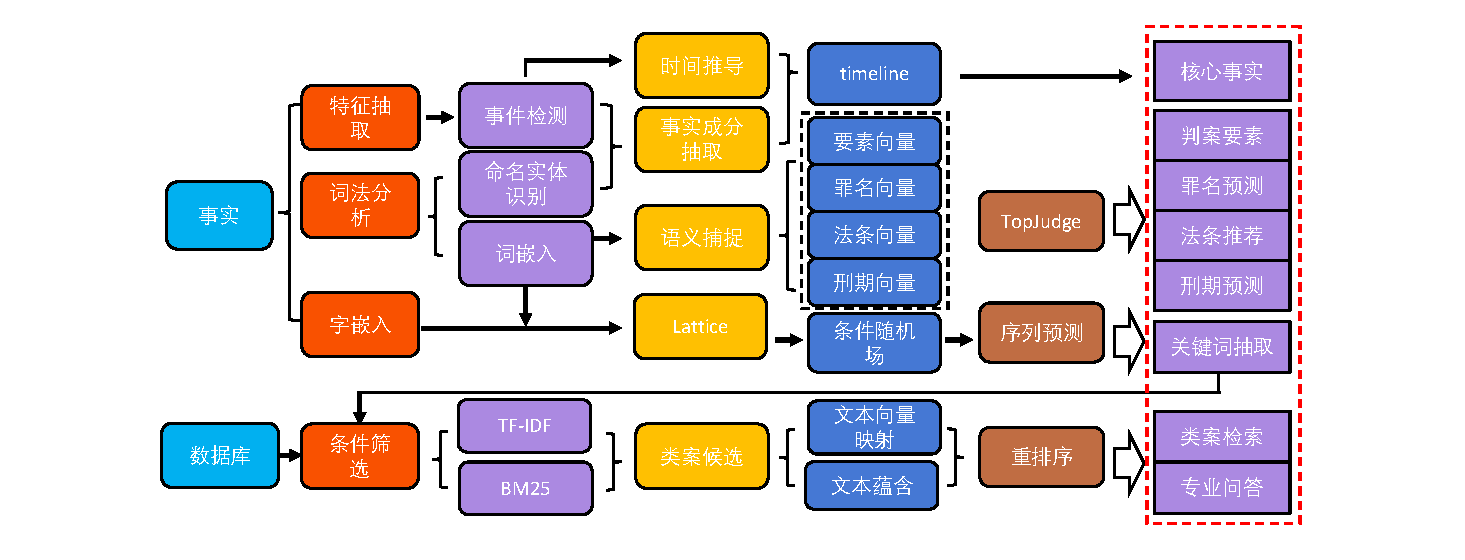
\includegraphics[width=\linewidth]{figures/flowsheet}
    \caption{平台工作流程图}
    \label{fig:flowsheet}
\end{figure*}


\section{成果概述}

通过长时间的努力,团队取得了许多阶段性成就。

\begin{enumerate}[1)]
	\item 多个司法智能领域的公开数据集。通过长时间的实践探索,在确定了每一个任务的规范流程之后,团队通过自动抽取、人工标注等多种方式构造了多个大规模公开数据集,其中包括多任务判决预测数据集,关键词抽取数据集,类案检索数据集,有效地推动了领域学术发展。
	\item 团队提出了要素式多任务判决模型,有效解决了数据分布长尾问题、罪名混淆问题、结果矛盾问题。并以此为基础申请科技发明专利一篇:“基于多任务学习的要素式法律案情分析方法”。
	\item 团队提出了基于栅栏式记忆神经网络的关键词抽取模型,解决了传统关键词抽取模型对词法分析工具的依赖导致的错误累积问题,申请科技发明专利一篇:“一种基于栅栏式长短时记忆神经网络的法律关键词抽取系统”。
	\item 团队提出了一种基于语言模型的语义相似检索算法,有效解决传统基于词语匹配的搜索引擎无法捕捉文本语义、无法克服语言差异的问题,申请科技发明专利一篇:“一种基于语言模型和词法分析的类案匹配算法”。
\end{enumerate}

\iffalse
\begin{enumerate}[1)]
	\item 大规模的法律文书数据集,通过长时间分布式的数据抓取,我们最终获得了数千万的法律文书,其中包括刑法500余万份;

	\item 关键词抽取数据集,为了实现关键词抽取模型,我们整理了10000份待标注的法律相关句子,通过专业人士的人工标注,我们最终获得了这样一份高质量的关键词抽取数据集;

	\item 判决预测模块算法的实现,提出了一个新的多任务学习模型,取得了很好的效果;

	\item 关键词模块算法的实现,将目前自然语言处理领域最前沿的序列标注模型应用至关键词抽取任务上,通过特征工程等方法,对算法进行了改进;

	\item 类案推荐搜索引擎的实现,提出两步走的检索算法,做到了语义相似性检索;

	\item 平台搭建,将所有算法集成到demo平台上,形成一个可用的法律产品。
\end{enumerate}
\fi

\begin{figure*}[ht]
    \centering
    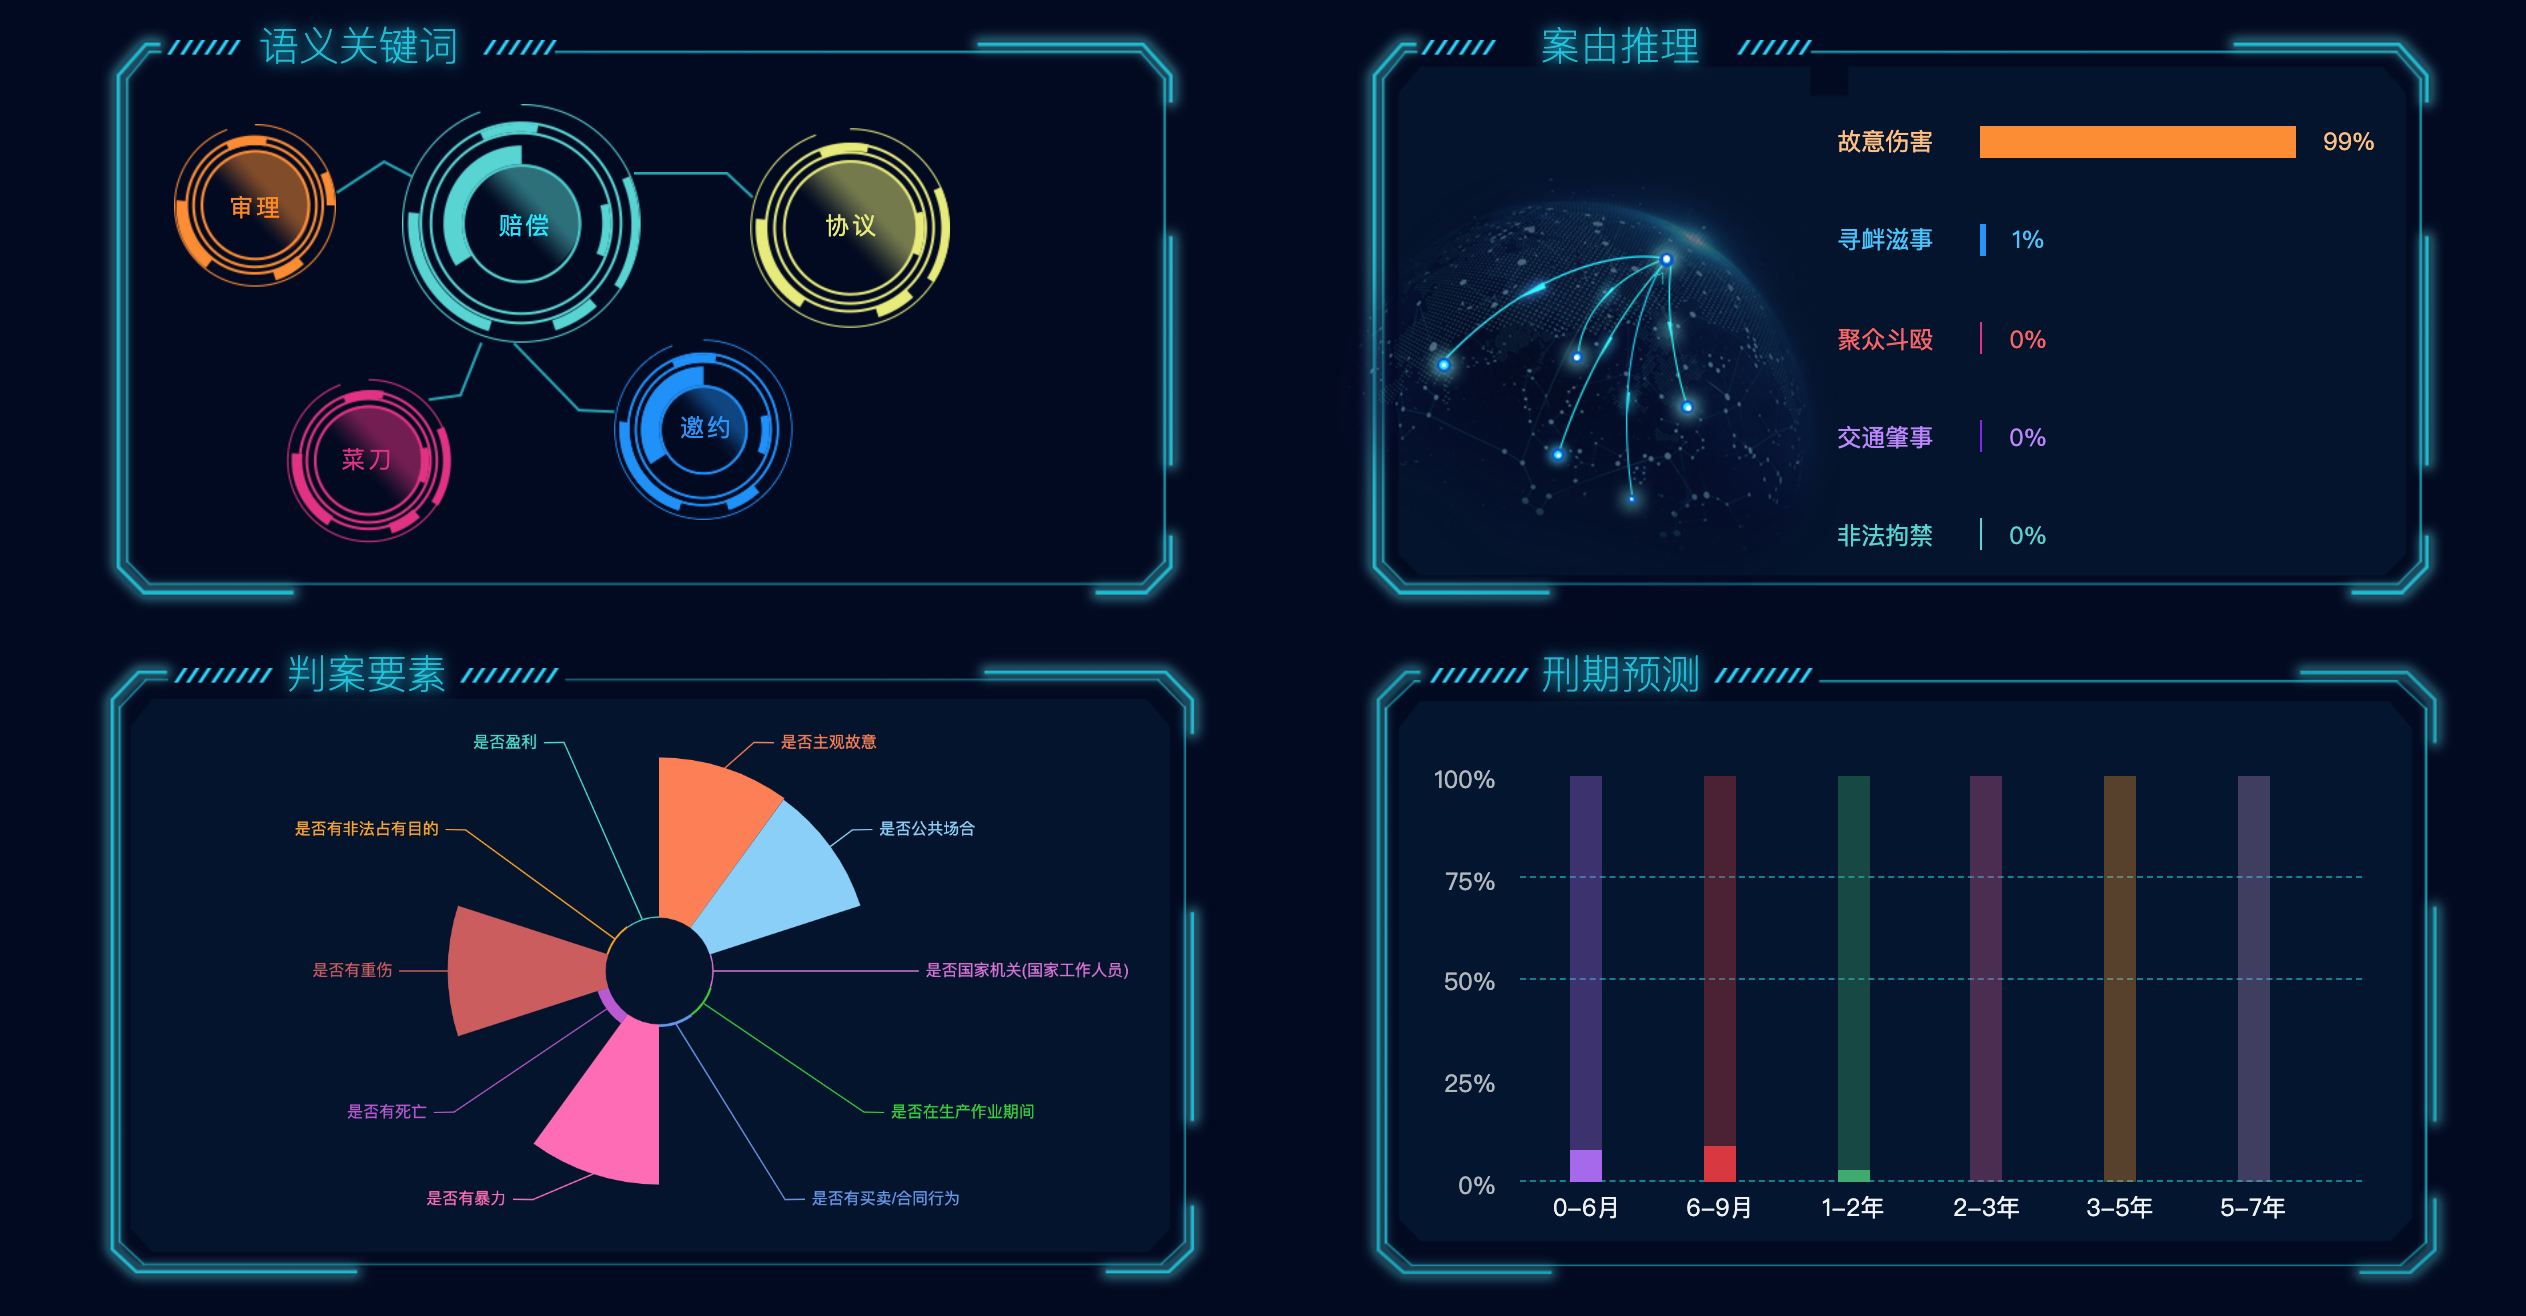
\includegraphics[width=\linewidth]{figures/demo.png}
    \caption{平台功能示意图}
    \label{fig:demo}
\end{figure*}
